\section{Matchings and Colorings}


\subsection[Matchins 1]{Prove that a $(2k+1)$-regular graph $\mathcal{G}$ with edge-connectivity $\lambda(G) \geq 2k$ has a perfect matching}

\vspace{3pt}

First we will start with the definition of edge-connectivity and a reminder of a theorem (Tutte) we will use to prove the statement.

\begin{definition}[Edge Connectivity]
    Given a graph $G$, it's edge connectivity, $\lambda(G)$ is the minimum number of edges whose deletion disconnect G.
\end{definition}

From the definition, it is clear that $\lambda(G) \leq \delta(G)$, which in our case implies $2k \leq \lambda(G) \leq 2k + 1$. To see the former, if we remove all the incident vertices to the vertex of smallest degree, we disconnect $G$, proving to be an upper bound.

\begin{theorem}[Tutte]
    Let $G = (V, E)$ be a graph. For every $S \subset V$ let $c_o(G - S)$ denote the number of odd components of $G[V-S]$. The graph $G$ contains a perfect matching if and only if, for every $S \in V(G)$,
    $$c_o(G-S) \leq |S| $$
\end{theorem}
we denote the latter condition as the Tutte condition.

Further, let us make the following observation on $G$'s cardinality, where we use the Handshaking lemma and the fact that $G$ is $(2k + 1)$-regular.
$$2|E(G)| = \sum_{v \in V(G)} d(v) = |V(G)|(2k + 1) \Rightarrow |V(G)| \equiv 0 \mod 2$$

Knowing that the cardinality is even, lets us easily check that Tutte's condition holds if $|S| = 0$. From now on we will then assume $|S| > 0$. Again, using $G$'s regularity, the following inequality holds:
\begin{equation}\label{edge-ineq}
\#\lbrace\text{edges incident to S from odd components}\rbrace \leq \#\lbrace\text{edges incident to S}\rbrace \leq |S|(2k + 1)
\end{equation}

Let now $C$ be an odd component of $G - S$. If we count all the vertices incident to some vertex of $C$, we have from one side the $(2k + 1)$ regularity, and from the other the edges within $C$ (beginning and end inside C) and those leaving $C$. By construction, all edges leaving C must necessarily be incident to $S$ (see the supporting drawing). Hence, the following holds:
$$|C|(2k + 1) = 2|E(C,C)| + |E(C,G-C)| = 2|E(C,C)| + |E(C,S)|$$

\begin{figure}[h!]
    \centering
    \resizebox{.8\linewidth}{!}{
        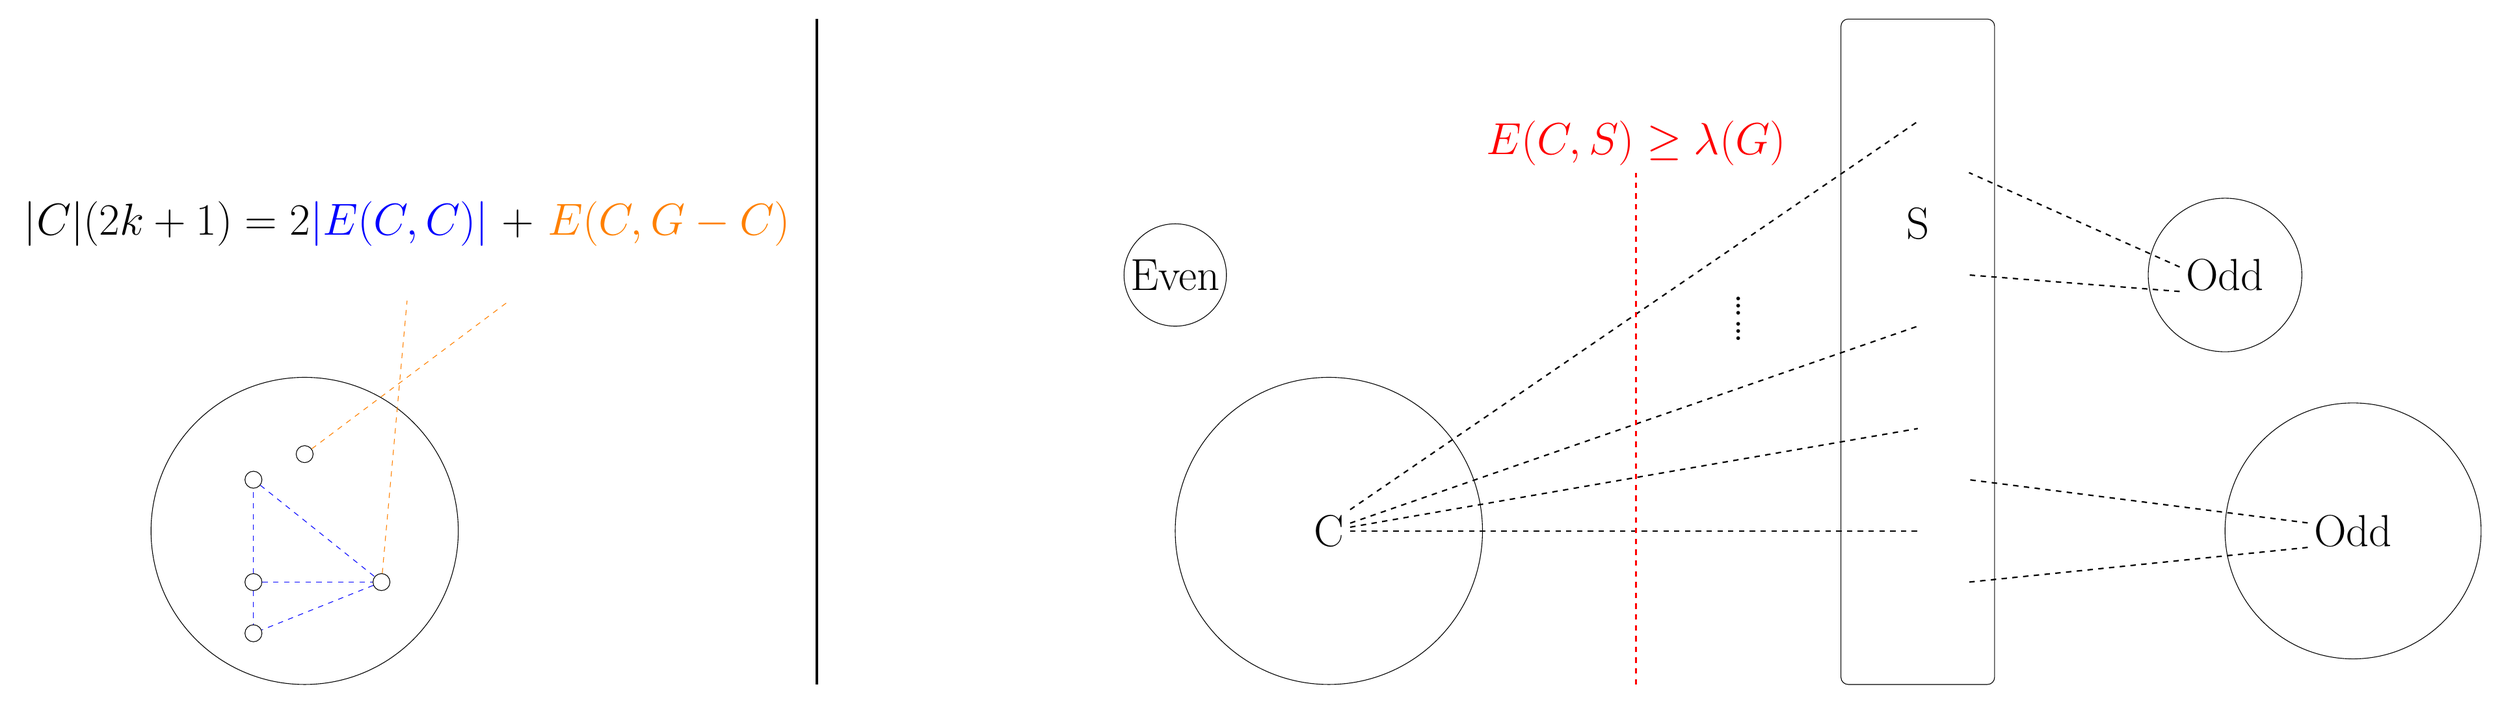
\begin{tikzpicture}
            % LHS Drawing
            \draw (0,0) circle (3cm);
            \node[circle, draw = black] (node-1) at (-1,-1) {};
            \node[circle, draw = black] (node-2) at (-1,1) {};
            \node[circle, draw = black] (node-3) at (1.5,-1) {};
            \node[circle, draw = black] (node-4) at (-1,-2) {};
            \node[circle, draw = black] (node-5) at (0,1.5) {};
            \draw[dashed, blue] (node-1) -- (node-2);
            \draw[dashed, blue] (node-1) -- (node-3);
            \draw[dashed, blue] (node-1) -- (node-4);
            \draw[dashed, blue] (node-2) -- (node-3);
            \draw[dashed, blue] (node-3) -- (node-4);
            \draw[dashed, orange] (node-3) -- (2,4.5);
            \draw[dashed, orange] (node-5) -- (4,4.5);
            \node at (2, 6.0) {\Huge $|C|(2k + 1) = 2$\textcolor{blue}{$|E(C,C)|$} + \textcolor{orange}{$E(C, G-C)$}};

            % Separating Line
            \draw[very thick] (10, -3) -- (10, 10);

            % RHS Drawing
            \draw (20, 0) circle (3cm) node (C) {\Huge C};
            \draw (17, 5) circle (1cm) node {\Huge Even};
            \draw[rounded corners] (30, -3) rectangle (33, 10);
            \node at (31.5, 6) {\Huge S};
            \draw(40, 0) circle (2.5cm) node (N1) {\Huge Odd};
            \draw(37.5, 5) circle (1.5cm) node (N2) {\Huge Odd};
            \draw[dashed, thick] (C.0) -- (31.5, 0);
            \draw[dashed, thick] (C.10) -- (31.5, 2);
            \draw[dashed, thick] (C.20) -- (31.5, 4);
            \draw[dashed, thick] (C.45) -- (31.5, 8);
            \draw[dashed, thick] (N2.200) -- (32.5, 5);
            \draw[dashed, thick] (N2.170) -- (32.5, 7);
            \draw[dashed, thick] (N1.200) -- (32.5, -1);
            \draw[dashed, thick] (N1.170) -- (32.5, 1);
            \node at (28, 4.5) {\Huge $\vdots$};
            \node at (28, 4) {\Huge $\vdots$};
            \draw[very thick, red, dashed] (26, -3) -- (26, 7) node[text=red,anchor=south] {\Huge $E(C, S) \geq \lambda(G)$};
        \end{tikzpicture}
    }
\end{figure}

Moreover, from the previous equality we observe that LHS has the parity of $|C|$, and the RHS has the parity of $|E(C,S)|$. Thus, $|C|$ and $|E(C,S)|$ have the same parity. In particular, $|E(C,S)|$ is odd. Lastly, given that $S$ disconnects $G$, by definition of edge connectivity we have
$$|E(C,S)| \geq \lambda(G) = \lbrace 2k, 2k + 1 \rbrace \overset{|E(C,S)| odd}{\Longrightarrow} |E(C,S)| \geq 2k + 1$$

Inserting this last inequality to (\ref{edge-ineq}) we have:
$$c_o(G-S)(2k + 1) \leq \#\lbrace\text{edges incident to S from odd components}\rbrace \leq |S|(2k + 1) \Rightarrow c_o(G-S) \leq |S|$$
which is exactly Tutte's condition, and hecne $G$ contains a perfect matching.

\newpage

\subsection[Matchings 3]{Show that the edges of a regular bipartite graph can be decomposed into pairwise disjoint matchings.}

Let $G$ be a $k$-regular bipartite graph, and let $X$ and $Y$ the left and right vertex sets.
Note that $k$-regularity implies $|X| = |Y|$.
Now consider $S \subset X$, $k|S| = |N(S)| \subset Y$.
Let us recall Hall's theorem:
\begin{theorem}[Hall]
    Let $G = (X \cup Y, E)$ be a bipartite graph.
    There is a matching $M$ in $G$ covering all vertices of $X$ if and only if for every $U \subset X$ we have
    $$ |N(U)| \geq |U| $$
\end{theorem}
It is clear that $S > |N(S)|$ implies that there is a vertex with cardinality greater than $k$ (not possible) hence $S \leq N(S)$ and we have a matching (in fact, a perfect one) in $G$.

Let us remove the edges corresponding to this matching, and we have a $k-1$-regular graph.
We progress similarly until we have our edge partition.

\newpage

\subsection[Matchings 6]{Show that a graph $G$ of order $n$ contains $\frac{n-k}{2}$ independent edges if and only if for every $S \subset V(G)$, it holds that}
$$c_o(G-S) \leq |S| + k$$

Let us consider $S > 0$, otherwise the statement trivially holds.

\begin{remark}
    An independent edge set of a graph $G$ is a subset of the edges such that no two edges in the subset shares a vertex of $G$.
\end{remark}

\begin{itemize}
    \item[$(\Rightarrow)$] We argue by contrapositive.
        $c_o(G-S) > |S| + k$ implies that there are at least $k+1$ more odd components than elements in $S$.
        This in turn means that, at most, we would have an $(n - k -1)$-matching from the odd components to $S$.
    \item[$(\Rightarrow)$] Let us build $G'$ such that $V(G') = V(G) \cup \{v_1, \dots, v_k \}$, we add $k$ new vertices connected to all vertices in $G$.
        Let us now observe that, for all $S' \subset V'$:
        \begin{enumerate}
            \item If $\exists v_i \: | \: v_i \not\in S'$ then $G'$ is connected and $c_o(G' - S') < 1 \leq |S'|$.
            \item If $\{ v_1, \dots, v_k \} \subseteq S' \Rightarrow S' = \{v_1, \dots, v_k \} \cup S$ for some $S$ in $G$.
                Then:
                $$c_o(G' - S') = c_o(G - S) \leq |S| + k = |S'|$$
        \end{enumerate}
        (1) and (2) prove that $G'$ satisfies the Tutte condition, and hence there exists a $n$-matching in $G'$, hence we have an $(n-k)$-matching in $G$ as we wanted to prove.
\end{itemize}

\newpage

\subsection[Matchings 9]{Show that (i) $\chi(G\square H) = \max\{\chi(G),\chi(H)\}$ and (ii) $\chi(G\times H) = \max\{\chi(G),\chi(H)\}$}

\begin{itemize}
    \item[(i)] Let us first observe that $G, H \subseteq G \square H$ and that $A \subseteq B \Rightarrow \chi(A) \leq chi(B)$.
        Therefore it is clear that $\max\{\chi(G), \chi(H)\} \leq \chi(G \square H)$.

        Secondly, $u$ and $v$ are adjacent in $G \square H$ if they agree on one coordinate and are adjacent in the other one, then $f(u,v) = \chi(u) + \chi(v) \mod \max\{\chi(G), \chi(H)\}$ is a proper coloring.
    \item[(ii)] We know that a graph is $k$-colorable if and only if it has an homomorphism to $K_k$. 
        Observe that $G \times H$ has clear homomorphisms (projections) to $G$ and $H$ and hence it exists an homomorphism $G \times H$ to $K_k$ and $K_g$.
        Thus, the coloring number is the minimum of the two.
\end{itemize}
